\documentclass[12pt]{article}
\usepackage{mathtools}
\usepackage{multicol}
\usepackage{float}
\usepackage[margin=1in]{geometry}
\usepackage{setspace}
\usepackage{mathrsfs}
\usepackage{gensymb}
\usepackage{fancyhdr}
\usepackage{graphicx}
\usepackage{indentfirst}
\usepackage{wrapfig} 
\usepackage{subfig}

\begin{document}
\section*{\centering Group 4 - UAV Project}
\begin{center} Peter Hartford, Julia Dunlop, Zixin Chen, Trevor Burgoyne\\
 Fall 2021\\
 \end{center}
\hrulefill
\subsection*{\centering Executive Summary} 

The goal of the UAV Obstacle Course project was to simulate the flight of an Unmanned Aerial Vehicle (UAV) to a series of way-points through an obstacle course filled with cubes and hoops. The UAV’s flight was scored based on whether it hit all of the way-points, went through any of the hoops, and if it hit any obstacles. Functions for plotting the UAV’s obstacle course were provided, as were the steering functions used to direct the UAV to the way-points.

Separate functions were assigned to individuals to write. Once finished, the project was troubleshooted as a group. A GitHub repository was created to keep track of file updates. UAVContol, UAVFlyThrough, UAVFlyToWayPoint, UAVFlyWayPointSequence, stopSim, ODENumIntRK4 and UAVRHS were the functions that were written to get the simulation to work. PlotUAVObstacleCourse to ensure that the simulation was run smoothly as well. \\


\begin{wrapfigure}{L}{0.5\textwidth}
	\begin{center}
		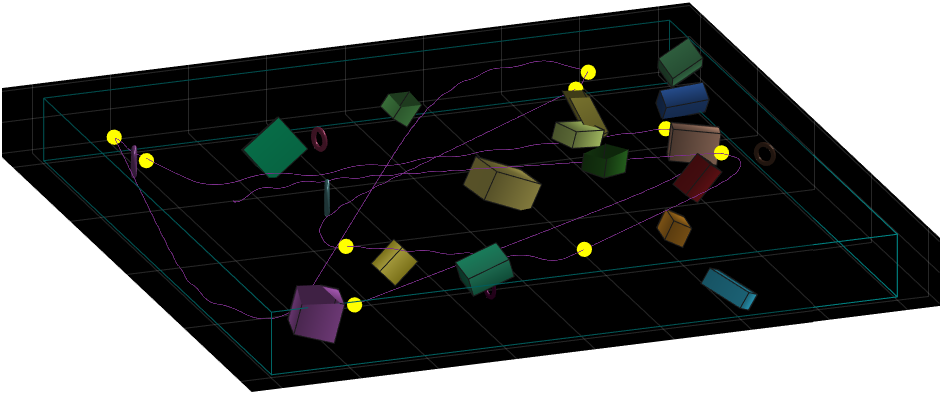
\includegraphics[scale=0.5]{Course1Traj}
		\caption{UAV Trajectory Through Course 1}
	\end{center}
\end{wrapfigure} 

Aside from following the project instructions, a few features were added to the simulation to make sure the UAV could get to each way-point. Inside UAVControl, limits were applied to the bank angle, normalized lift and normalized thrust. Not only do those limits more accurately represent an actual flight, they made the simulation run smoother and kept the all values as real numbers. Adding additional way-points made it easier for the UAV to fly to each required way-point, as it wasn’t trying to turn quite so hard. In UAVRHS, limits were applied to the UAV to keep it within the boundaries of the obstacle course. 

Figure 1 shows the simulation of the UAV through Course 1 with additional way-points. Running the course through the scoring function obtains an overall score of 100 points. The UAV makes it through 1 hoop, but hits 1 cuboid. 	




\pagebreak
\subsection*{\centering Summary of Roles}  

\begin{description}
\item[Julia Dunlop:] Wrote the UAVControl and added limits to UAVRHS to keep UAV inside course. Wrote the majority of the executive summary. 

\item[Zixin Chen:] Wrote the entire RHS function. Revised and made extra comments on the code.

\item[Peter Hartford:] Wrote the ODENumIntRK4 function, formatted the executive summary, and wrote the main report. Edited some of the course data to increase the score of the UAV

\item[Trevor Burgoyne:] Meshed the functions together to get the simulation to work. Edited the parameters of the UAVControl function to get it to output reasonable values.

\end{description}

\pagebreak  
\subsection*{\centering Report} 
A dynamic model was provided to help with the creation of the UAVRHS function. 
The simulation was run on three different courses and scored using the ScoreUAVObstacleCourse function. For each course, the UAV path was scored on the number of cuboids and way-points the UAV hit, and if it flew through any of the hoops. Each of the paths and scores for the obstacle courses are outlined below. 
\begin{figure}[H]
	\subfloat[1][Plotted Trajectories for Course 1]{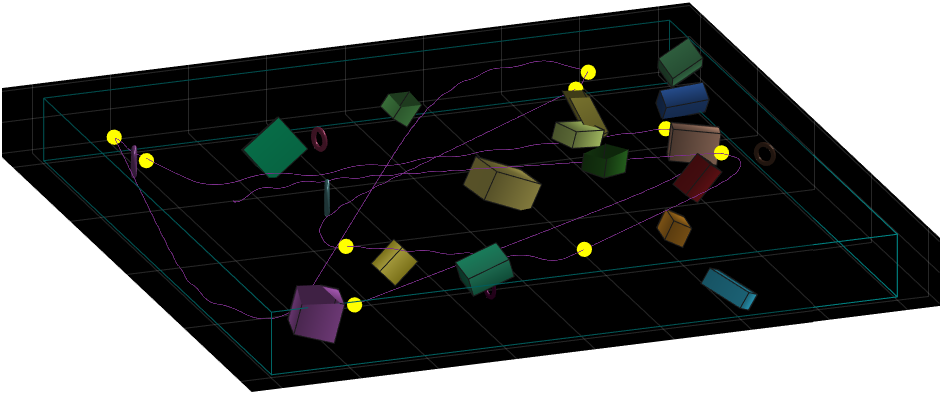
\includegraphics[scale=0.5]{Course1Traj}}
	\subfloat[2][Scoring for Course 1 (note the one red box that was hit)]{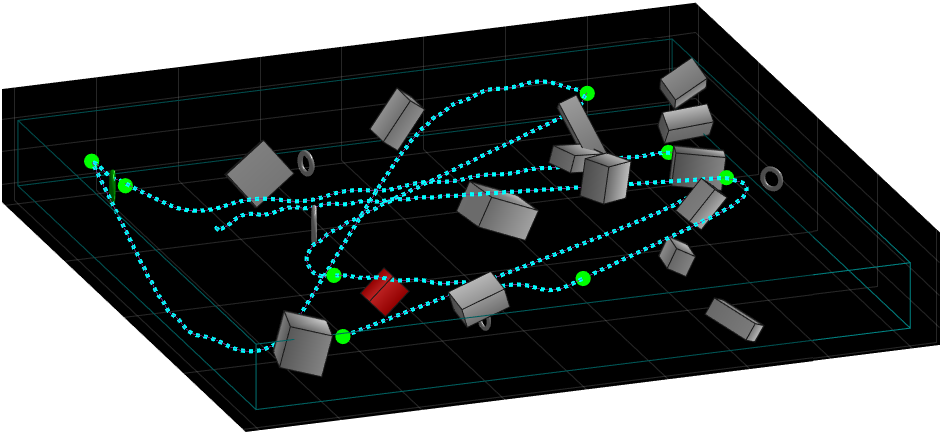
\includegraphics[scale=0.5]{Course1Score}}
	\caption{Trajectories and scoring for Course 1}
\end{figure}
Figure 2-a shows the simulated trajectory for the UAV using some of the predetermined way-points for Course 1. The UAV was easily able to fly to all of the way-points, achieving a score of 1000 points because it ended up hitting one of the cuboids, but it was able to fly through one of the hoops. Figure 2-b illustrates the two targets that changed the UAV's score. The hoop is highlighted in green, and the box is highlighted in red. 
\begin{figure}[H]
	\subfloat[1][Plotted Trajectories for Edited Course 1]{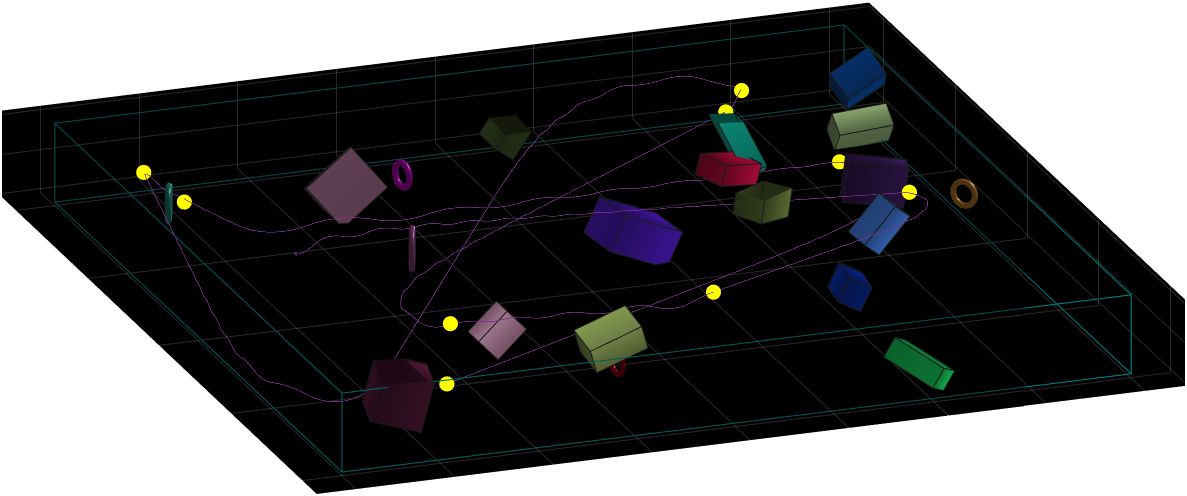
\includegraphics[scale=0.4]{Course1NewTraj}}
	\subfloat[2][Scoring for Edited Course 1 (note no boxes were hit!)]{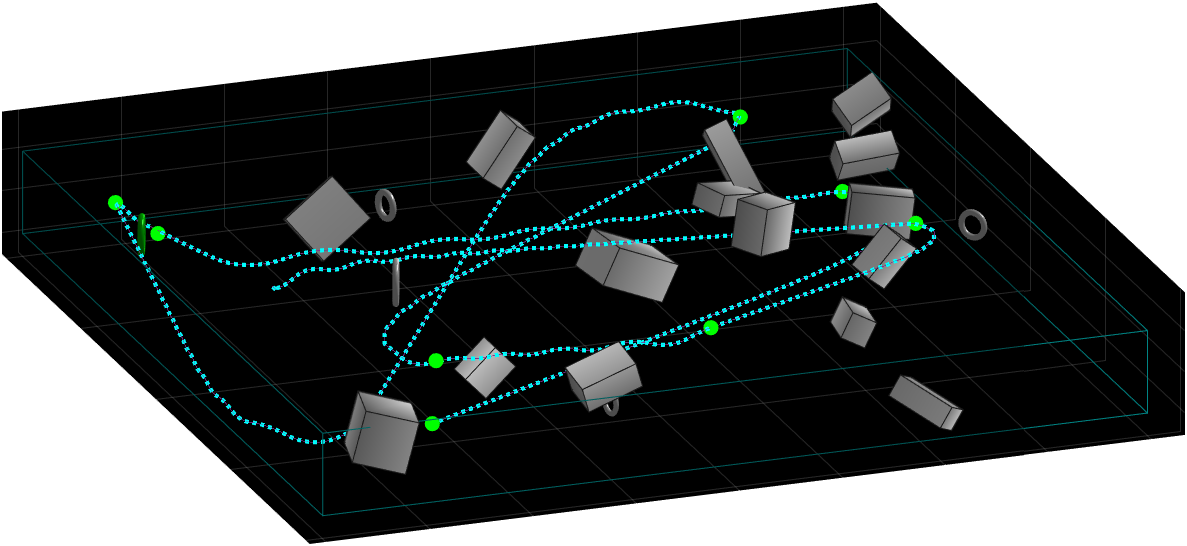
\includegraphics[scale=0.4]{Course1NewScore}}
	\caption{Trajectories and scoring for an Edited Course 1}
\end{figure}
Figure 3-a shows the same course with the way-points slightly shifted to make it so the UAV did not hit any of the boxes. With this new regime, the UAV hit all of the way-points and achieved a score of 1050 because it also went through one of the hoops. This is clearly illustrated in Figure 3-b with no red boxes and one green hoop. 
\begin{figure}[H]
	\subfloat[1][Plotted Trajectories for Course 2]{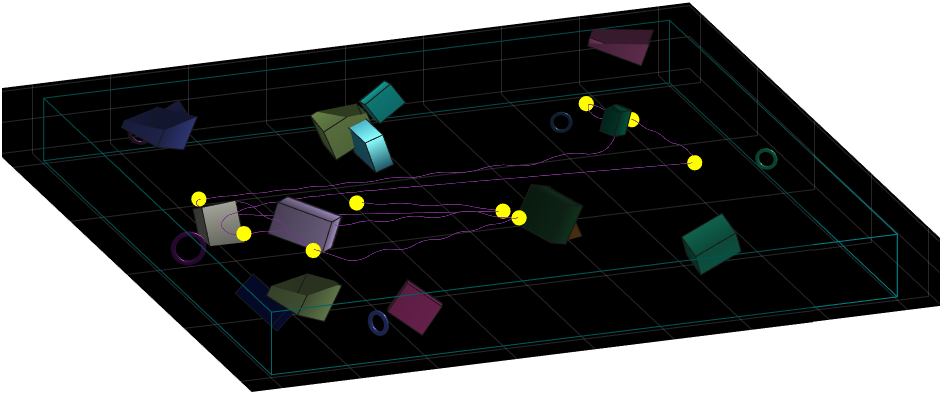
\includegraphics[scale=0.5]{Course2Traj}}
	\subfloat[2][Scoring for Course 2 (note the two red boxes that were hit)]{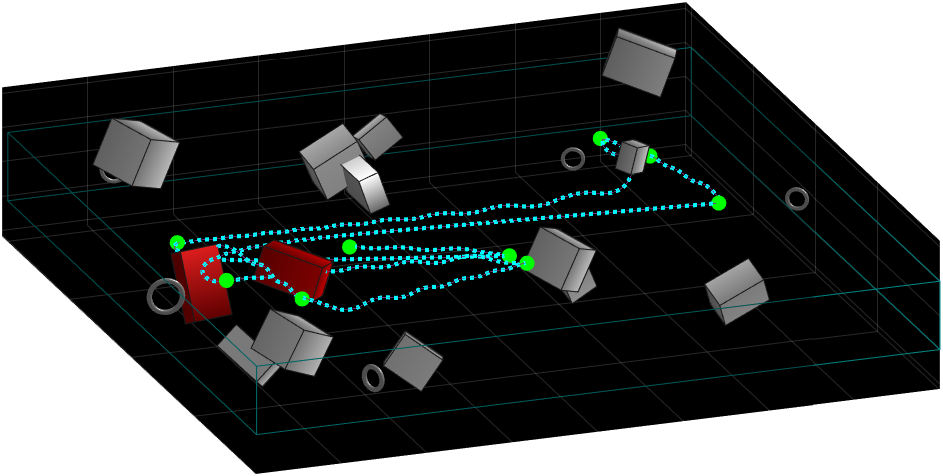
\includegraphics[scale=0.5]{Course2Score}}
	\caption{Trajectories and scoring for Course 2}
\end{figure}
Figure 4-a shows the simulated trajectory for the UAV using some of the predetermined way-points for Course 2. The UAV was easily able to fly to all of the way-points, achieving a score of 900 points because it ended up hitting two of the cuboids. Unfortunately, the UAV was not able to fly through any hoops, so it ended up having the worst score  Figure 4-b illustrates the two targets that changed the UAV's score. The two boxes that were hit are relatively close to each other, and could possibly be avoided by changing the way-points. 
\begin{figure}[H]
	\subfloat[1][Plotted Trajectories for Course 3]{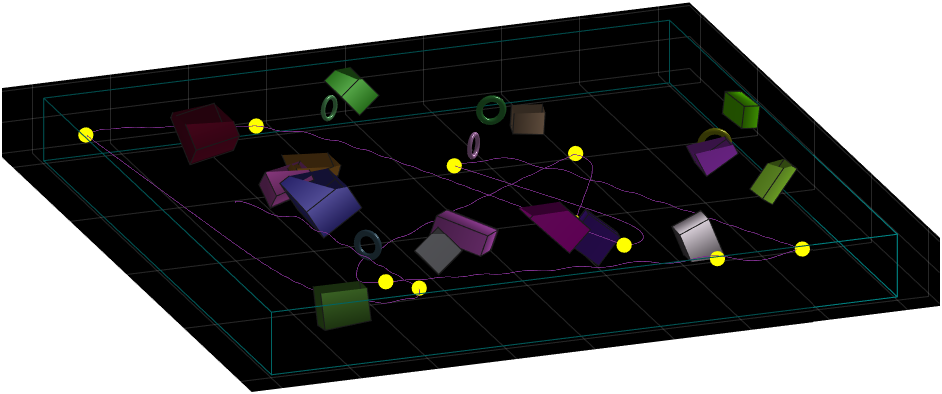
\includegraphics[scale=0.5]{Course3Traj}}
	\subfloat[2][Scoring for Course 3 (note the one red box that was hit)]{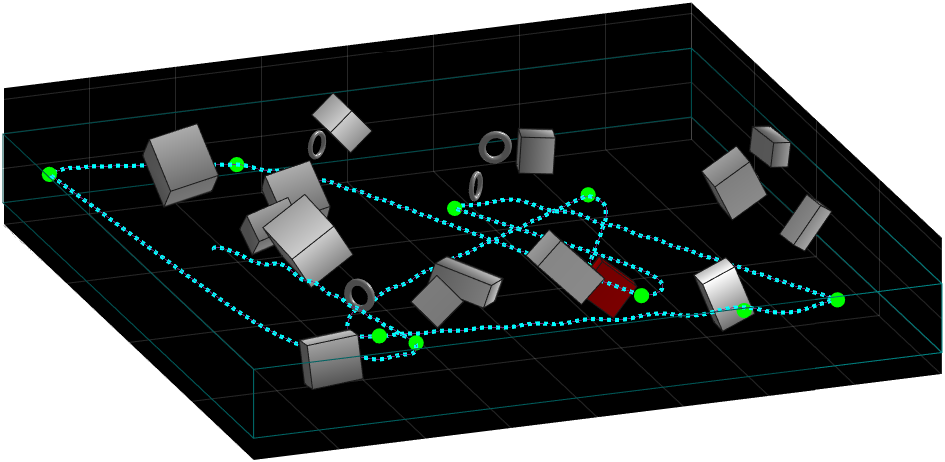
\includegraphics[scale=0.5]{Course3Score}}
	\caption{Trajectories and scoring for Course 3}
\end{figure}
Figure 5-a shows the simulated trajectory for the UAV using some of the predetermined way-points for Course 3. The UAV was easily able to fly to all of the way-points, achieving a score of 950 points because it ended up hitting one of the cuboids. Unfortunately, the UAV was not able to fly through any hoops. Figure 5-b illustrates the one target that changed the UAV's score. The box that was hit is highlighted in red. 
\\

The task of simulating the UAV simulation required a few functions to be written and modified in order for it to work properly. A brief description of each of the written functions is as follows: 
\begin{description}
	\item[PlotUAVObstacleCourse] takes in a way-point list, initializes the state vector, control gains, UAV parameters, engine time response, then calls UAVFlyWaypointSequence.
	\item[UAVFlyWaypointSequence] loops through each way-point to set parameters for each segment between those way-points and calls UAVFlyToWayPoint
	\item[UAVFlyToWaypoint] sets a time interval for the segment and calls 
	UAVSim. 
	\item[UAVSim] calls UAVGuidance, which calculates the required state for the UAV to get to the next way-point. 
	\item[UAVControl] takes the current state, commanded state and gain parameters and outputs the required bank angle, normalized lift, and normalized thrust.
	\item[UAVRHS] contains the dynamic model outputting the state derivatives, and is called after UAVControl inside UAVSim. The state is then updated and then the next time step is simulated. 
	\item[stopSim] breaks UAVSim when the UAV is incapable of reaching the way-point due to control limits, or if the UAV passes through the way-point. 
\end{description}

The control limits were edited to ensure that the UAV was ran through the course in a realistic manner. The engine response time was changed from 5 seconds to 5 miliseconds becuause there were issues with the UAV not responding in a quick enough manner. The maximum lift ($L_{max}$) was changed to 10 Newtons because there were issues with the UAV not having enough lift to complete the course. 

\end{document}